\shorthandoff{"}
\chapter{Diskussion}
\label{ch:diskussion}

\section{Zusammenfassung der Forschungsergebnisse}
\label{ch:diskussion:zusammenfassung}
Im Rahmen der vorliegenden Master-Thesis wurde eine Fallstudie unter Projektmanagern und Mitarbeitern des IT-Beratungsunternehmens EXXETA AG durchgeführt. Dabei wurden die Vorschläge zur Besetzung offener Projektpositionen eines uni- und eines bilateralen Empfehlungsansatzes miteinander verglichen. Das bilaterale Vorschlagsverfahren konnte bei vier der fünf evaluierten Stellen eine höhere Zufriedenheit bei den Angestellten erzielen. Bei einer Projektposition sorgte dagegen der unilaterale Empfehlungsansatz für eine höhere Zufriedenheit. Vergleichbar fielen auch die Ergebnisse auf Seiten der Projektmanager aus. Hier prognostizierten die Verantwortlichen für drei der fünf Projektpositionen eine höhere Arbeitsleistung von den vorgeschlagenen Mitarbeitern des bilateralen Verfahrens. Bei zwei Stellen bewerten die Projektmanager dagegen die Arbeitsleistungen der vorgeschlagenen Angestellten der unilateralen Variante als höher.

Bei grafischer Darstellung von Präferenzen und beherrschten Fähigkeiten der befragten Mitarbeiter zeigte sich der sogenannte lange (Ratten-)Schwanz. Zudem hatten 17 Prozent der Angestellten keine einzige Kompetenzbewertung im Intranet der EXXETA AG vorgenommen. Darüber hinaus konnte festgestellt werden, dass die Mitarbeiter einen Großteil ihrer präferierten Fähigkeiten nicht beherrschen. Weitere Analysen ergaben, dass etwa 28 Prozent aller Angestellten eine Fähigkeit nicht als Präferenz angaben, obwohl sie diese beherrschen. 

Abschließend wurde evaluiert, wie Mitarbeiter und Projektmanager mit möglicher Unterforderung bei der Projektarbeit umgehen. Diesbezüglich konnte im Rahmen der Befragung festgestellt werden, dass sowohl Angestellte als auch Projektverantwortliche mehrheitlich eine Unterforderung vermeiden möchten.

\section{Interpretation der Forschungsergebnisse}
\label{ch:diskussion:interpretation}
In Kapitel \ref{ch:personEnvironmentFit:auswirkungenErhoehterAngebote} wurde beschrieben, dass ein P-E Misfit in drei möglichen Konsequenzen mit entsprechenden Gleichungen zur Berechnung resultieren kann. Im Rahmen der vorliegenden Master-Thesis wurde angenommen, dass sowohl Projektmitarbeiter als auch -manager eine Unterforderung bei der Besetzung offener Projektpositionen vermeiden möchten. Dementsprechend wurde Kurve B aus Abbildung \ref{fig:personEnvironmentFit:auswirkungenErhoehterAngebote:abb1} in Form der quadrierten Differenzberechnung implementiert. Die im Rahmen der Fallstudie erhobenen Daten bestätigen diese Annahme sowohl aus Perspektive der Mitarbeiter als auch aus dem Blickwinkel der Projektverantwortlichen. 

Bei Implementierung der beiden Empfehlungsansätze wurde aufgrund der Erkenntnisse aus Kapitel \ref{ch:empfehlungssysteme} erwartet, dass der lange (Ratten-)Schwanz und der Kaltstart die Vorschlagserstellung beeinträchtigen werden. Daher lag sowohl der uni- als auch der bilateralen Empfehlungsmethode ein hybrider und graphenbasierter Ansatz zugrunde, welcher über die Einbeziehung von Fähigkeitsbewertungen und Teamzuordnungen beide Probleme löste. Dieses Vorgehen ist mit Blick auf die Auswertung von beherrschten und präferierten Kompetenzen der Mitarbeiter als sinnvoll zu bewerten. Einerseits konnte in Abbildung \ref{fig:ergebnisse:analyse:abb1} der lange (Ratten-)Schwanz identifiziert werden. Andererseits hatten 17 Prozent der Mitarbeiter im Intranet keine einzige Fähigkeit bewertet. Folglich wären diese Angestellten ohne Einbeziehung der Teamzuordnungen von einem Kaltstart betroffen.

Hinsichtlich der Kompetenzen konnte außerdem beobachtet werden, dass die Mitarbeiter einen Großteil ihrer präferierten Fähigkeiten nicht beherrschen. Aus diesem Sachverhalt lässt sich schließen, dass die Angestellten bereit sind, in Zukunft weitere Fähigkeiten zu erlernen und diese bei der Projektarbeit anzuwenden. Auf Unternehmensseite könnte dementsprechend der Einsatz zusätzlicher Weiterbildungsangebote evaluiert werden, bei welchen die Mitarbeiter nicht nur bestehende Kompetenzen vertiefen, sondern auch neue Fähigkeiten erlernen können.

Des weiteren zeigte die Auswertung der Mitarbeiterkompetenzen, dass das Beherrschen einer Fähigkeit keinen Rückschluss auf eine entsprechende Präferenz zulässt. Ein unilateraler Empfehlungsansatz würde dennoch sämtliche beherrschten Kompetenzen gleich behandeln. Somit ist davon auszugehen, dass die Angestellten bei Einsatz eines unilateralen Empfehlungssystems für Projektpositionen vorgeschlagen werden, deren gesuchte Fähigkeiten diese zumindest teilweise nicht anwenden möchten. Ein bilaterales System unterscheidet dagegen zwischen präferierten und nicht gewünschten Kompetenzen. Da dieser Ansatz präferierte Fähigkeiten stärker gewichtet, wird sich ein vorgeschlagener Mitarbeiter mit höherer Wahrscheinlichkeit die Anwendung der geforderten Kompetenzen wünschen. Dementsprechend ist eine höhere Zufriedenheit und Motivation bei der Stellenbesetzung zu erwarten. Diese Annahme spiegelt sich auch in den Ergebnissen der Umfragen unter den Mitarbeitern und Projektmanagern der EXXETA AG wider. Zur Verdeutlichung dieses Sachverhalts zeigt Abbildung \ref{fig:diskussion:interpretation:abb1} erneut die prognostizierte Zufriedenheit der Mitarbeiter mit den fünf vordefinierten Projektpositionen aus Kapitel \ref{ch:ergebnisse:fallstudie:umfrageMitarbeiter}.

\begin{figure}[h]
	\centering
	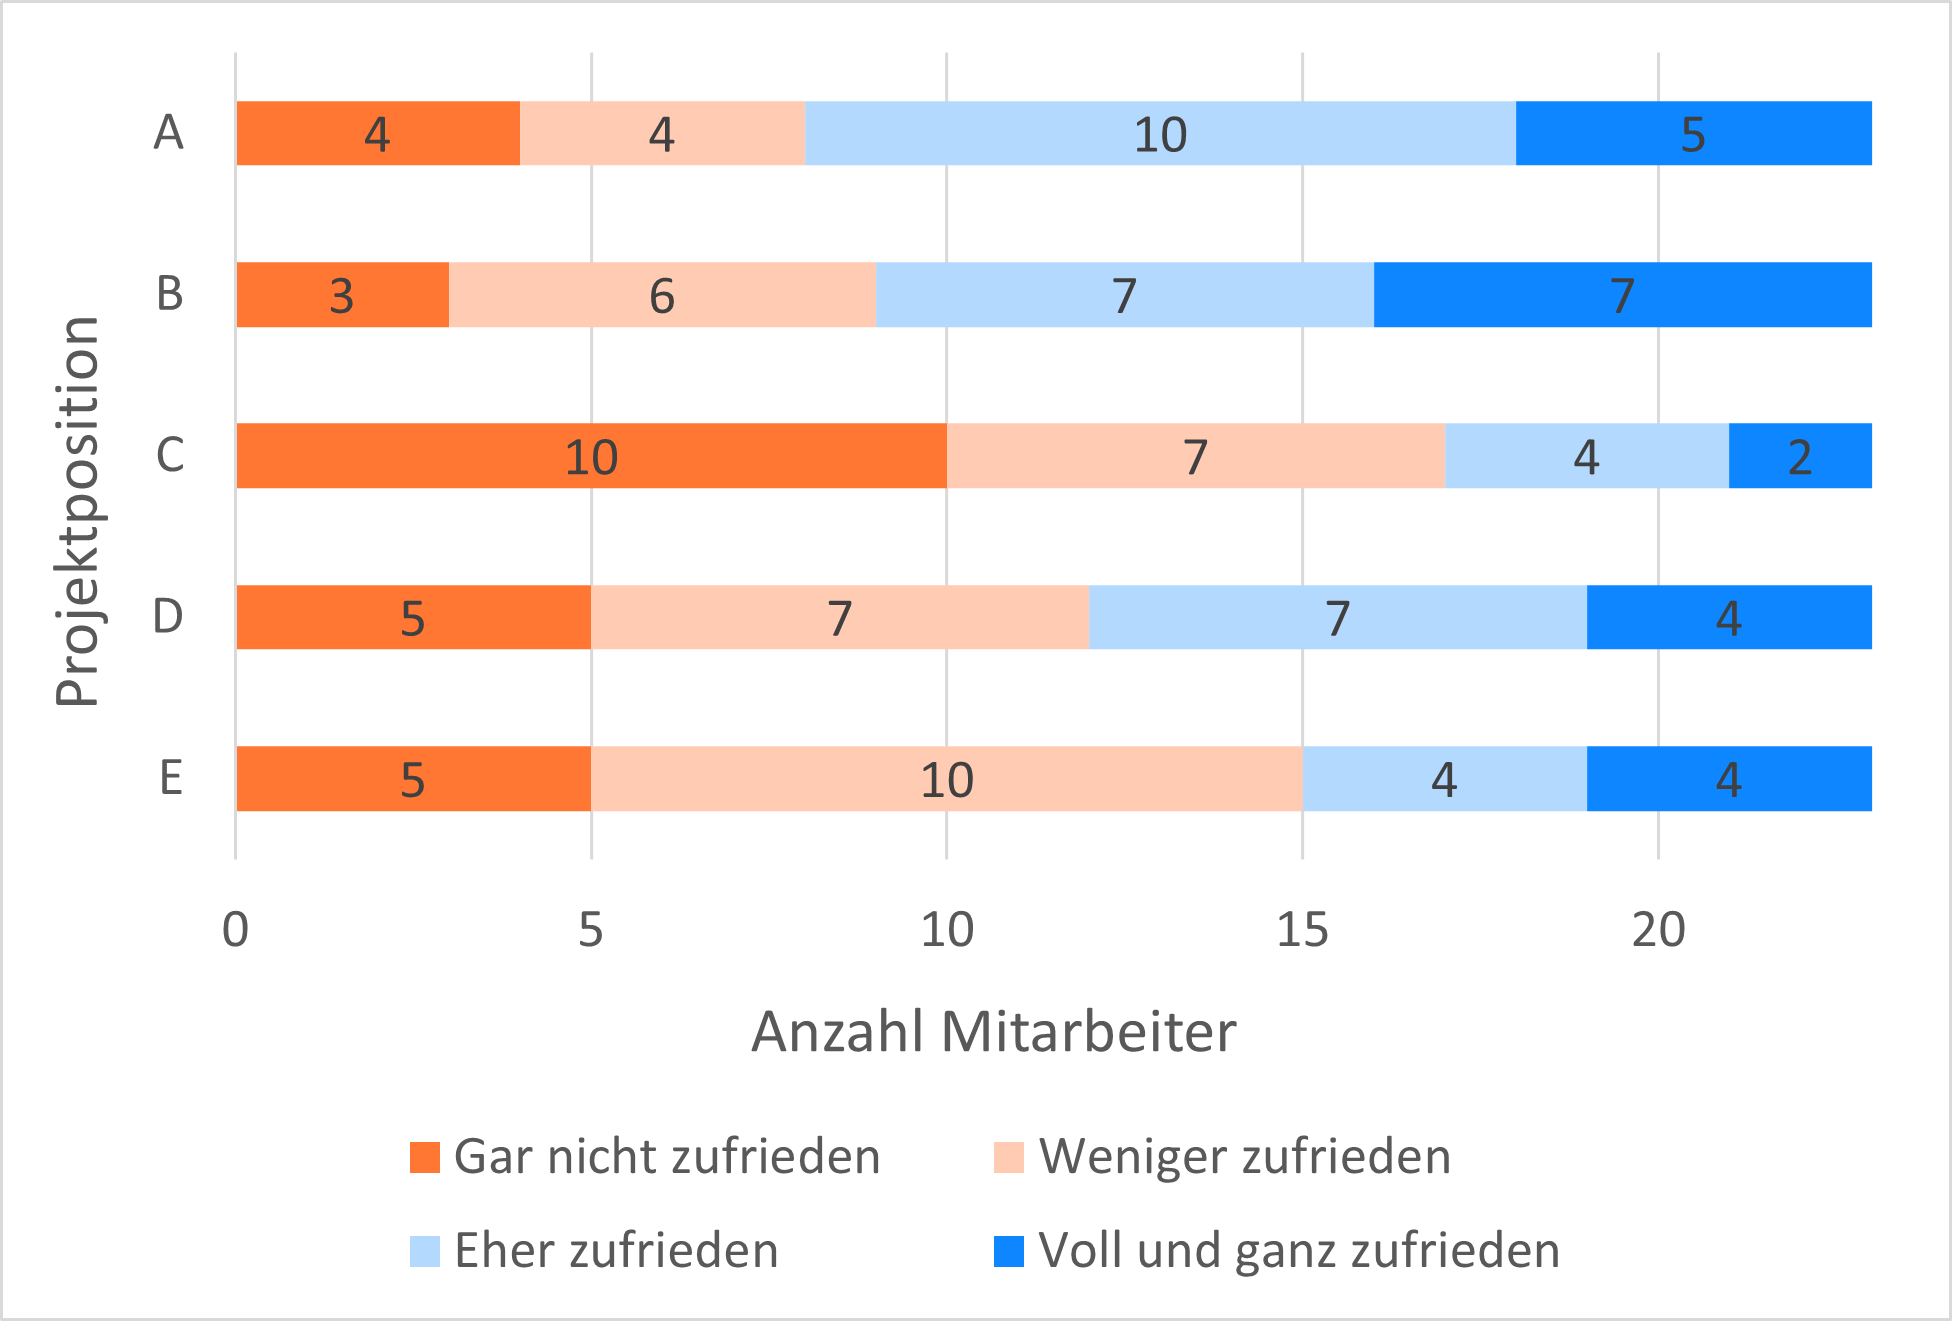
\includegraphics[width=0.8\textwidth]{gfx/mitarbeiter-zufriedenheit-umfrage.png}
	\caption{Anzahl an Mitarbeitern, welche zufrieden bzw. unzufrieden mit der Tätigkeit auf den jeweiligen vordefinierten Projektpositionen wären}
	\label{fig:diskussion:interpretation:abb1}
\end{figure}

Abbildung \ref{fig:diskussion:interpretation:abb3} veranschaulicht zusätzlich die Ergebnisse der uni- und bilateralen Empfehlungsansätze hinsichtlich der Mitarbeiterzufriedenheit. 

\begin{figure}[h]
	\centering
	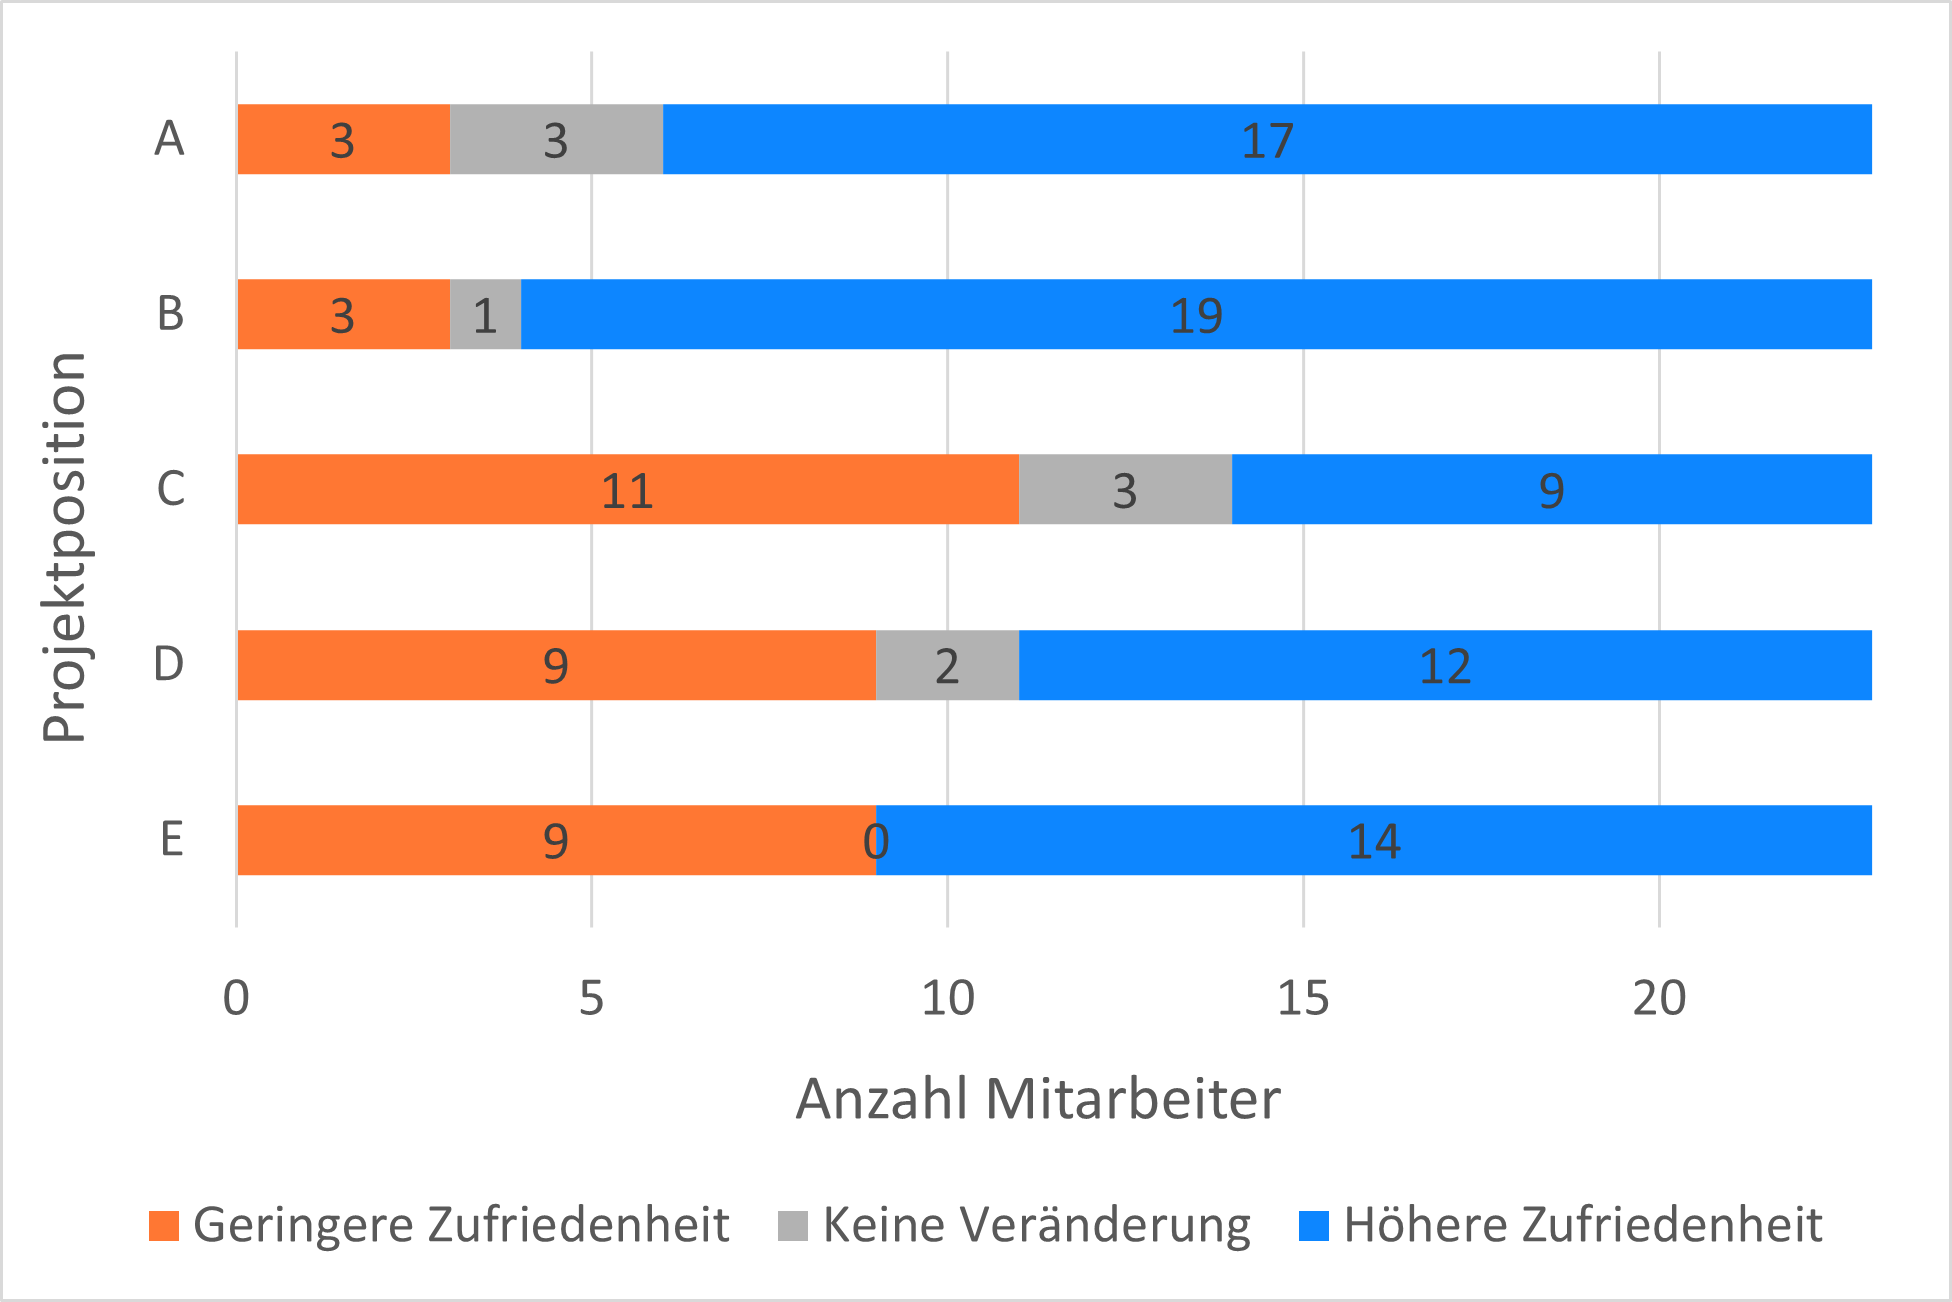
\includegraphics[width=0.8\textwidth]{gfx/zufriedenheit-projekte.png}	
	\caption{Ergebnisse des bilateralen Empfehlungsansatzes im Vergleich zum unilateralen Vorgehen hinsichtlich der Mitarbeiterzufriedenheit}
	\label{fig:diskussion:interpretation:abb3}
\end{figure}

In den Abbildungen \ref{fig:diskussion:interpretation:abb1} und \ref{fig:diskussion:interpretation:abb3} ist zu erkennen, dass die Mitarbeiter durch den bilateralen Empfehlungsansatz stärker zu deren Zufriedenheit positioniert werden, wenn sie eine hohe Zufriedenheit mit der Stelle prognostizieren. Dieser Sachverhalt ist insbesondere bei den Projektpositionen A und B zu beobachten. Mit diesen zeigten sich über die Hälfte der Mitarbeiter in Abbildung \ref{fig:diskussion:interpretation:abb1} zufrieden. Hier ordnete der bilaterale Empfehlungsansatz in Darstellung \ref{fig:diskussion:interpretation:abb3} etwa dreiviertel aller Angestellten gegenüber den unilateralen Variante stärker zu deren Zufriedenheit an. Zeigen sich dagegen weniger Mitarbeiter mit einer betrachteten Stelle zufrieden, nimmt auch die Qualität des bilateralen Empfehlungsansatzes hinsichtlich der Mitarbeiterzufriedenheit ab. Besonders gut ist diese Begebenheit bei Projektposition C zu erkennen, mit welcher sich die Mitarbeiter in Abbildung \ref{fig:diskussion:interpretation:abb1} mehrheitlich unzufrieden zeigten. Hier erzielte der bilaterale Empfehlungsansatz in Grafik \ref{fig:diskussion:interpretation:abb3} im Vergleich zur unilateralen Variante sogar Ergebnisse, welche zu einer geringeren Zufriedenheit der Mitarbeiter führten. Ähnliche Ergebnisse können ebenfalls für die Perspektive der Projektmanager abgeleitet werden. Abbildung \ref{fig:diskussion:interpretation:abb4} zeigt die Resultate der Umfrage unter den Projektverantwortlichen hinsichtlich der erwarteten Arbeitsleistung der Angestellten.

\begin{figure}[h]
	\centering
	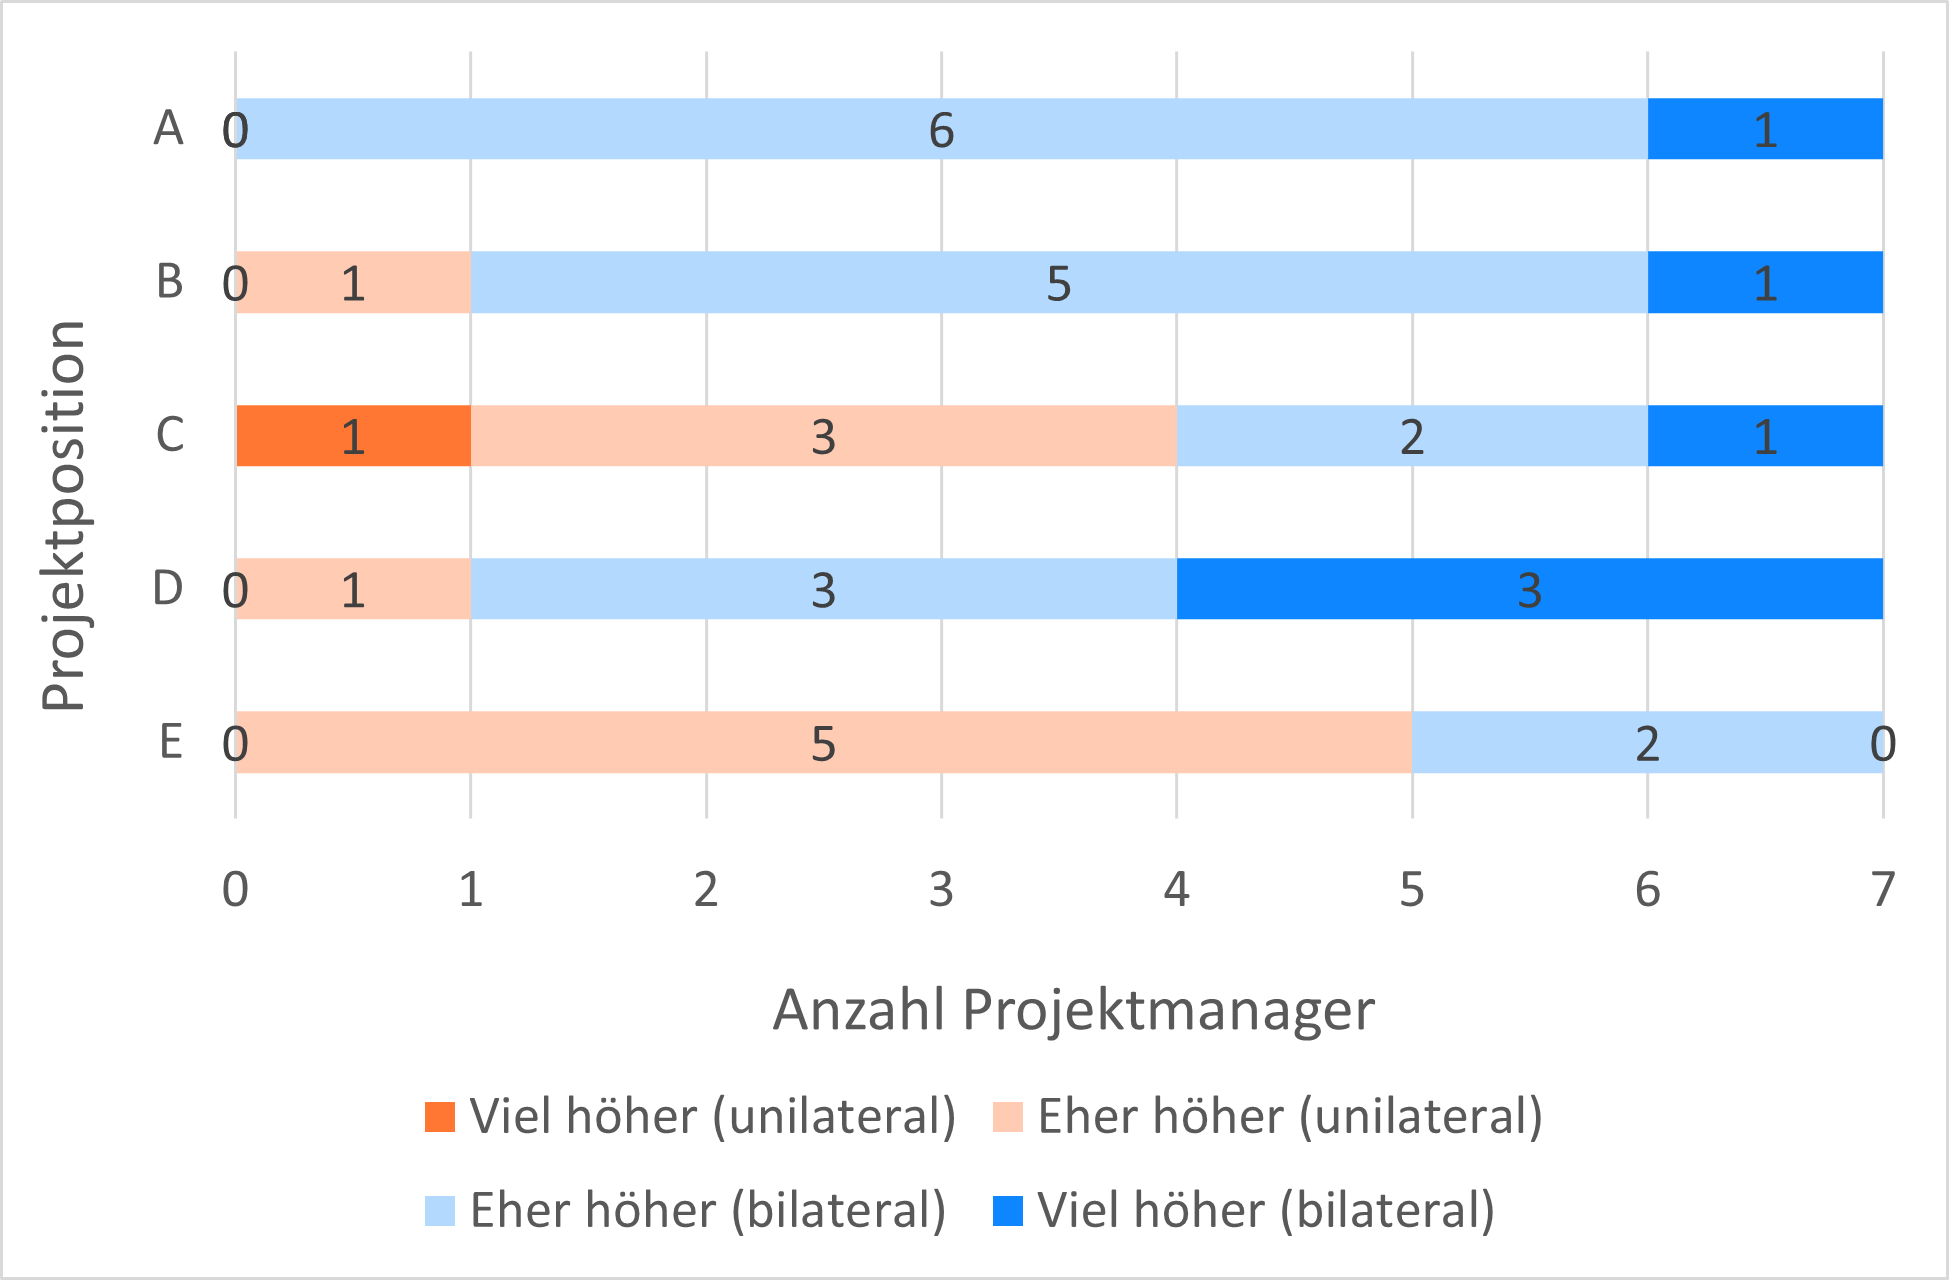
\includegraphics[width=0.8\textwidth]{gfx/ergebnisse-projektmanager-arbeitsleistung.png}	
	\caption{Ergebnisse der Umfrage unter den Projektmanager hinsichtlich der erwarteten Arbeitsleistung der Mitarbeiter}
	\label{fig:diskussion:interpretation:abb4}
\end{figure}

In Abbildung \ref{fig:diskussion:interpretation:abb4} ist für die Projektpositionen A und B zu beobachten, dass die Projektmanager eine höhere Arbeitsleistung von den Vorschlägen des bilateralen Empfehlungsansatzes erwarteten. Hierbei handelt es sich um die Stellen, mit welchen sich auch ein Großteil der Mitarbeiter in Abbildung \ref{fig:diskussion:interpretation:abb1} zufrieden zeigten. Für die Projektpositionen C und E, mit welchen die Angestellten in Darstellung \ref{fig:diskussion:interpretation:abb1} mehrheitlich unzufrieden waren, erwarteten die Projektmanager eine geringere Leistung von den Vorschlägen des bilateralen Empfehlungsansatzes.

Dementsprechend wird aus den Ergebnissen der Fallstudie geschlossen, dass der bilaterale Empfehlungsansatz im Vergleich zur unilateralen Variante immer dann für eine höhere Zufriedenheit bei den Angestellten und für eine gesteigerte erwartete Arbeitsleistung unter den Projektmanagern sorgt, wenn sich die Mitarbeiter mehrheitlich zufrieden mit der betrachteten Stelle zeigen. Eine Ausnahme von dieser Regel bildet lediglich Projektposition D in Abbildung \ref{fig:diskussion:interpretation:abb4}. Hier sorgten die Vorschläge des bilateralen Empfehlungsansatzes aus Perspektive der Projektmanager für eine wesentlich höhere prognostizierte Arbeitsleistung, obwohl sich die Mitarbeiter in Darstellung \ref{fig:diskussion:interpretation:abb1} mehrheitlich unzufrieden mit der Stelle zeigten. Wie in Abbildung \ref{fig:diskussion:interpretation:abb2} zu erkennen, unterschieden sich die Vorschläge zu Projektposition D in der Umfrage unter den Projektmanagern jedoch in nur einer Person.

\begin{figure}[h]
	\centering
	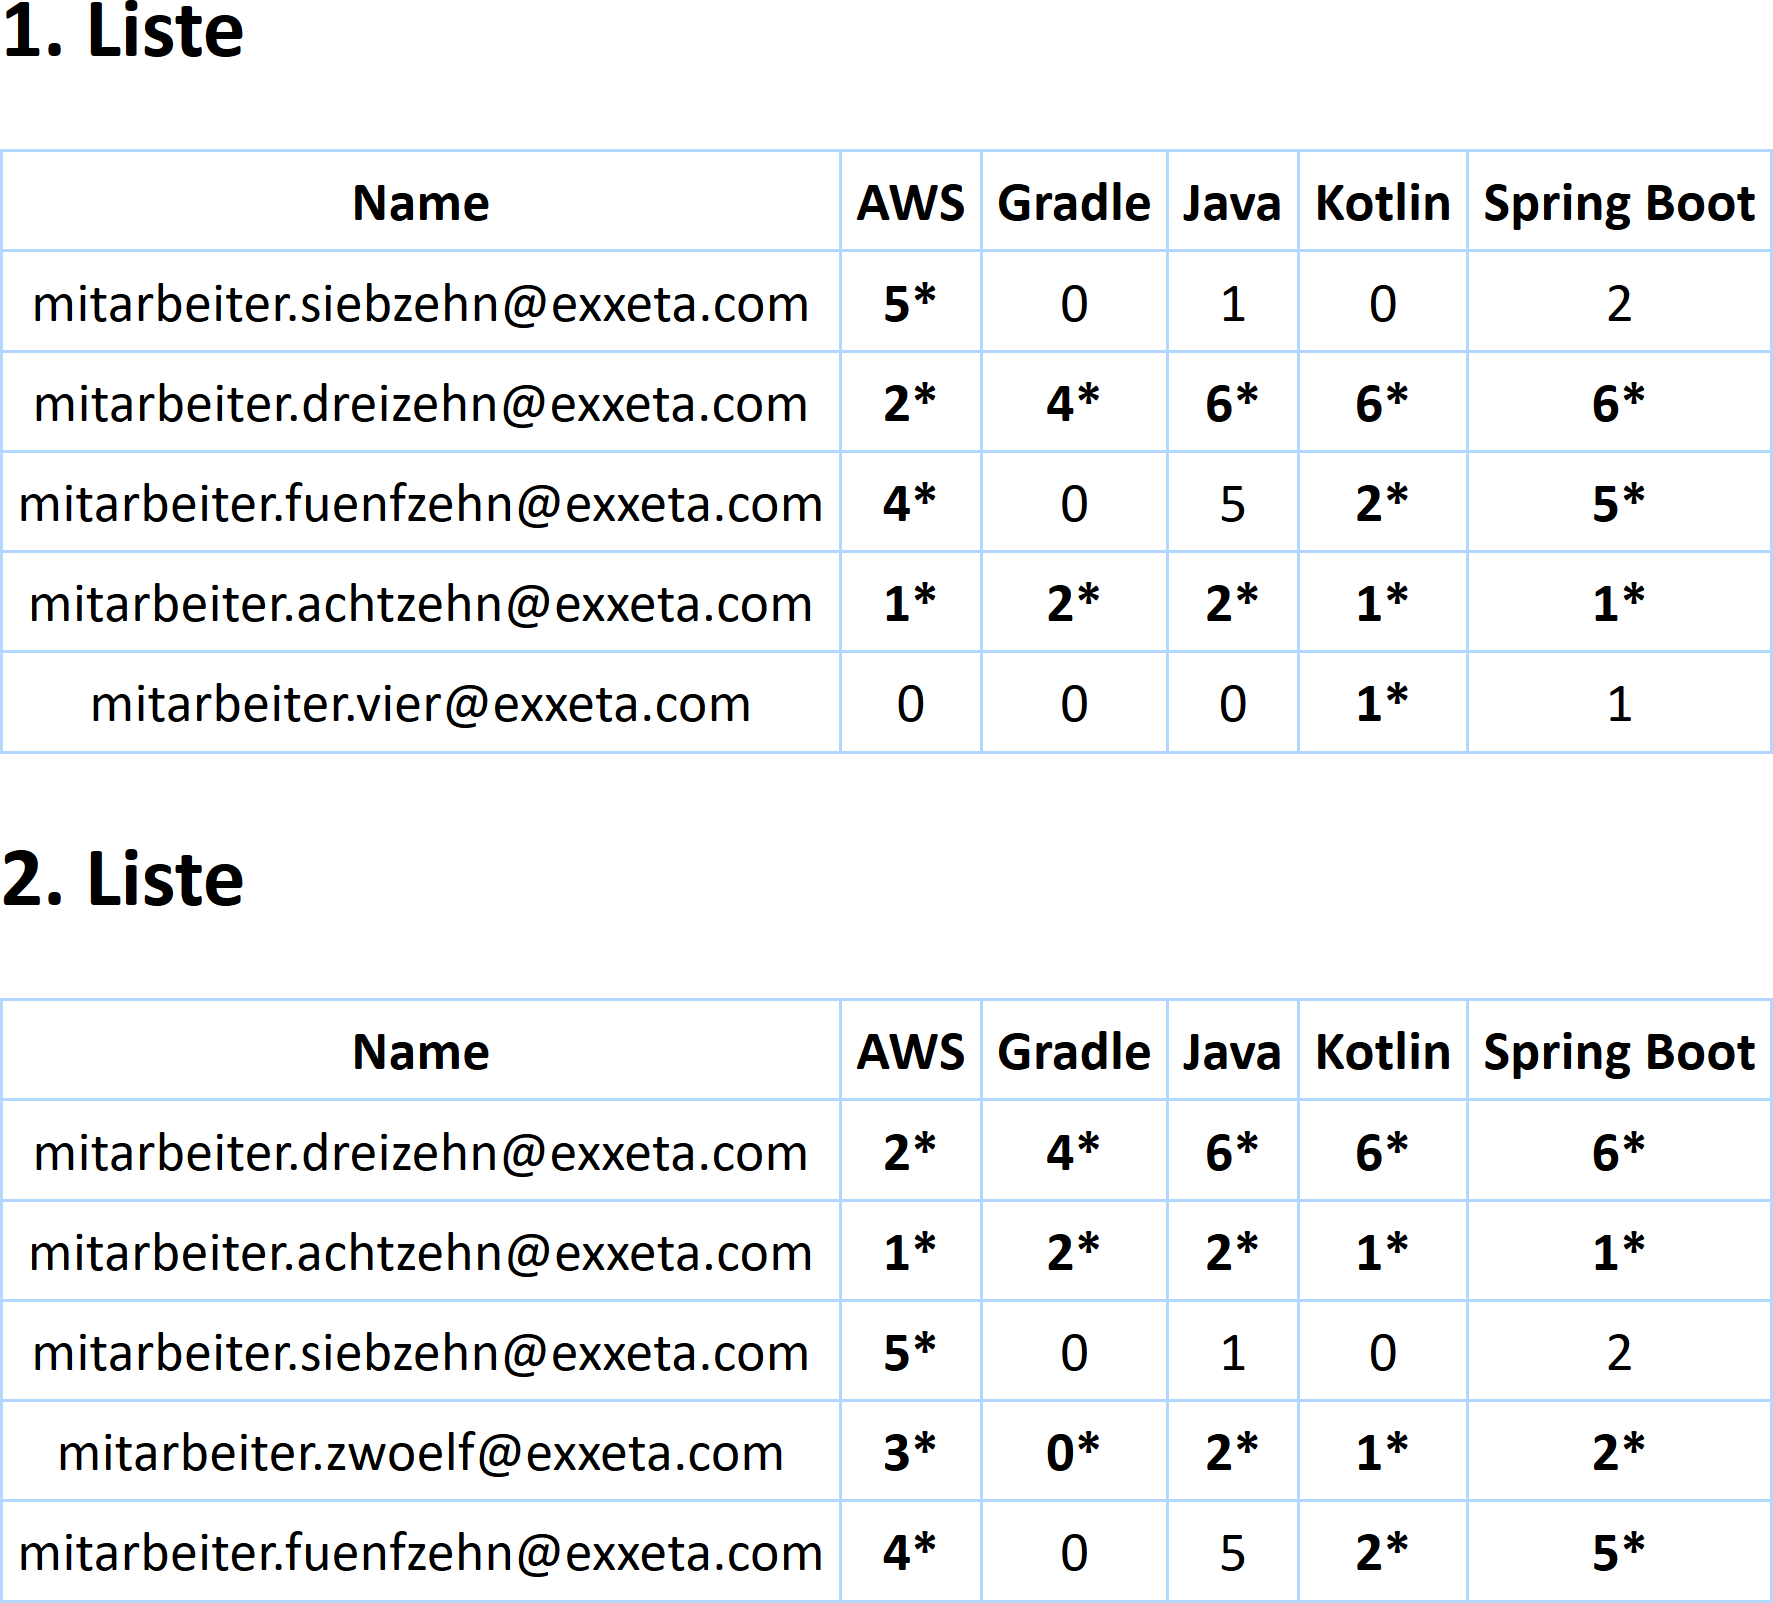
\includegraphics[width=0.75\textwidth]{gfx/projektposition-d.png}
	\caption{Mitarbeiter-Vorschläge für Projektposition D in der Umfrage unter den Projektmanagern\\
	(Klarnamen wurden aus Datenschutzgründen nachträglich pseudonymisiert)}
	\label{fig:diskussion:interpretation:abb2}
\end{figure}

Aufgrund des geringen Unterschieds in den Vorschlägen aus Abbildung \ref{fig:diskussion:interpretation:abb2} werden die Ergebnisse der Projektverantwortlichen für Projektposition D als nicht repräsentativ betrachtet, sodass sie die erlangten Erkenntnisse nicht widerlegen.

Somit ist zusammenfassend festzustellen, dass der bilaterale Empfehlungsansatz für eine höhere Zufriedenheit der Angestellten und eine gesteigerte Arbeitsleistung seitens der Projektmanager sorgt, wenn sich die Mitarbeiter mehrheitlich zufrieden mit einer betrachteten Projektposition zeigen.

Als Ursache für diese Einschränkung wird die Art der Erhebung der Präferenzen betrachtet. Die Mitarbeiter gaben im Rahmen der vorliegenden Master-Thesis ihre Wünsche über boolesche Werte an. Hierbei gewichtete der bilaterale Empfehlungsansatz die präferierten Fähigkeiten der Angestellten höher. Es wurde jedoch nicht unterschieden, ob ein Angestellter einer nicht gewünschten Kompetenz neutral gegenübersteht oder ob er diese nicht bei der Projektarbeit anwenden möchte.

Aufgrund dieser Einschränkung wird für folgende Arbeiten empfohlen, den im Rahmen dieser Arbeit implementierten Empfehlungsansatz zu erweitern. Hierbei sollten die Präferenzen nicht über boolesche Werte, sondern über Abstufungen der Form "möchte ich anwenden", "neutral", "möchte ich nicht anwenden" erhoben werden. Bei der Implementierung sollten die Mitarbeiter bei vorhandenem Wunsch weiterhin höher positioniert werden. Bei Angabe eines negativen Wertes sollten die Angestellten zusätzlich niedriger einsortiert werden. Unter Betrachtung dieser Veränderungen sollte die Evaluation unter Mitarbeitern und Projektmanagern nochmals durchgeführt und die Forschungsfrage entsprechend erneut untersucht werden.

\section{Einordnung in die Literatur und Ausblick}
\label{ch:diskussion:einordnung}
Bislang betrachten Empfehlungssysteme im Bereich der Personalauswahl Problemstellungen laut \textcite{malinowski:2008} zumeist entweder aus Perspektive der Personalsachbearbeiter oder aus dem Blickwinkel der Mitarbeiter. Dieses Vorgehen verfolgte im Rahmen der vorliegenden Arbeit auch die unilaterale Empfehlungskomponente. Diese betrachtete ausschließlich die Präferenzen und Spezifikationen der Projektmanager. Obwohl die bilaterale Variante zusätzlich die Wünsche der Mitarbeiter einbezog und somit die Vorschläge des unilateralen Systems verzerrte, verbesserten sich die gemessenen Ergebnisse für die Mehrheit der Projektpositionen sowohl auf Seiten der Mitarbeiter als auch auf Seiten der Projektmanager. Somit zeigt die vorliegende Arbeit, dass die Erkenntnisse von \textcite[S. 5ff.]{parsons:1909} aus dem Jahr 1909 bzw. \textcite[S. 11f.]{lewin:1936} und \textcite[S. 38ff.]{murray:1938} aus den 1930er-Jahren zum Zusammenwirken von Person und Umgebung noch heute aktuell sind und sich auch auf die Implementierung von Empfehlungssystemen übertragen lassen. Diese Erkenntnis sollten zukünftige Arbeiten bei der Entwicklung von Vorschlagsverfahren im Bereich der Personalauswahl berücksichtigen und ihren Fokus von der getrennten Betrachtung von Person und Umgebung verstärkt auf das Zusammenspiel beider Komponenten richten. 


\shorthandon{"}